\chapter{Fejlestimering} \label{fejlestimering} 

Når man omformer uendelig-dimensionelle problemer i form af
differentialligninger til et sæt af endeligt mange ligninger med
endeligt mange ubekendte, vil der uundgåeligt opstå nogle fejl. En stor
del af forskningsindsatsen indenfor den endelige element metode består
i at udvikle og dokumentere metoder til evaluering af den fejl, der
opstår i denne proces. I dette kapitel skal vi se nærmere på en hjørne
af fejlestimering.

\section{Generel teori om fejlestimering}
Før vi betragter en egentlig metode til fejlestimering, vil vi ganske
kort gøre nogle generelle betragtninger omkring fejlestimering.

\subsection{Beregningsmæssige- og modelleringsfejl}
Den fejl, som man begår ved at omformulere et differentiallignings
problem til et variations problem, kan opdeles i 
\begin{itemize}
  \item beregningsmæssige fejl.
  \item modelleringsfejl.
\end{itemize}
For at konkretisere disse fejl typer skal vi betragte en matematiske model
\begin{equation} \label{math-model}
  \D u=f,
\end{equation}
hvor $\D$ er en differentialoperator (muligvis med begyndelsesværdi-
eller rand\-be\-tin\-gel\-ser) defineret på et vist domæne $\dom$, $f$ en 
given funktion, og $u$ er den ukendte løsning til problemet. Den 
matematiske model består her af $\D$ og $f$. Udgangspunktet for den
matematiske model er typisk en fysisk model\footnote{Ved en fysisk
model forstås en model, der modellere en situation hentet fra fx
økonomi, kemi eller fysik.}
\begin{equation} \label{phys-model}
  \tilde{\D} \tilde{u} = \tilde{f}.
\end{equation}
Her har $\tilde{\D}$, $\tilde{u}$ og $\tilde{f}$ analoge betydninger.
Den fysiske model antages at have en entydig løsning, og vi skal
desuden antage, at den matematiske model er konstrueret udfra den
fysiske model på en sådan måde, at der ligeledes for denne findes en
entydig løsning. Lad nu $\uex$ være den eksakte løsning til
\eqref{math-model}, og lad $\ufe$ være en approksimeret 
løsning til \eqref{math-model} beregnet ved hjælp af den endelige 
element metode. Vi vil da definere den beregningsmæssige fejl som
\begin{equation}
  e_{\mathsf{c}} = \uex - \ufe\ .
\end{equation}
Er $\tilde{u}_{\mathsf{ph}}$ løsningen til \eqref{phys-model}, 
defineres modelleringsfejlen som 
\begin{equation}
  e_{\mathsf{m}} = \tilde{u}_{\mathsf{ph}} - \uex\ .
\end{equation}
Den samlede fejl defineres da som 
\begin{equation}
  e=\tilde{u}_{\mathsf{ph}}-\ufe=\tilde{u}_{\mathsf{ph}}-\uex+\uex-\ufe
  =e_{\mathsf{m}} + e_{\mathsf{c}}\ ,
\end{equation}
dvs. som summen af modelleringsfejlen og den beregningsmæssige fejl.
Vi skal her  kun beskæftige os med beregningsmæssige fejl. 

\subsection{Forskellige typer af fejlestimatorer}
Igennem årene er der blevet foreslået et utal at forskellige 
fejlestimatorer til brug i den endelige element metode, se fx
\cite{babuska1} for 
litteraturhenvisninger. Flertallet af disse fejlestimatorer kan 
klassificeres i en af følgende to kategorier:
\begin{itemize}
  \item Udglatnings metoder (eng. smoothening/flux-projection).
  \item Residuum metoder.
\end{itemize}
Vi skal i afsnit~\ref{z2} betragte en bestemt udglatnings metode.
Traditionelt set har residuum metoder haft størst udbredelse, men den
udglatnings metode, som vi senere skal studere, vil måske medvirke til at åbne
vejen for en større udbredelse af fejlestimatorer af denne type.
 
\subsection{Forskellige former for fejlestimering}
Man skelner normalt mellem to former for fejlestimering
\begin{itemize}
  \item A priori fejlestimering.
  \item A posteriori fejlestimering.
\end{itemize}
Ved a priori fejlestimering forsøger man at vurdere fejlen mellem den
eksakte løsning og den approksimerede løsning alene på grundlag af
egenskaberne ved den eksakte (ukendte) løsning til problemet. I a 
posteriori fejlestimering forsøger man derimod at vurdere fejlen vha. 
den beregnede approksimerede løsning. De to former for fejlestimering 
ses ofte anvendt i forskellige teoretiske og praktiske situationer. A
priori fejlestimering bruges typisk til at bestemme 
konvergensegenskaberne for den numeriske metode, mens a posteriori
fejlestimering ofte anvendes i adaptive algoritmer som en del af
netinddelings algoritmen og stopkriteriet.

Specifikke egenskaber ved fejlestimatorer er tæt knyttet til den 
type af differentialligninger, som de er konstrueret i tilknytning til. 
Af denne grund findes kun  meget få generelle teoretiske resultater om
fejlestimatorer. Til gengæld findes en del begreber og definitioner,
som man benytter, når man skal vurdere og/eller sammenligner en eller
flere fejlestimatorer. 

\subsection{Definitioner og begreber} \label{def-beg}
\begin{definition}
Ved en celle forstås en mindre samling af sammenhængende elementer, 
se figur \ref{fig-cell}. Bemærk at en celle godt kan bestå af et  
enkelt element.
\end{definition}
\begin{figure}[hbtp]
  \setlength{\unitlength}{1bp}
  \begin{center}
    \begin{picture}(169,155)(0,0)
      \put(1,1){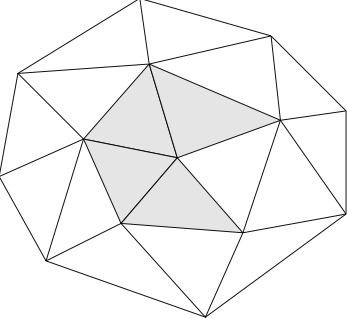
\includegraphics{cell}}
    \end{picture}
  \end{center}
  \caption{Eksempel på celle\label{fig-cell}}
\end{figure}
\begin{definition}
Lad $\dom$ betegne domænet, hvori vi ønsker at løse en given
differen\-tialligning, og lad $\T=\{\fee_k\}_{k=1}^N$ være en
triangulering af $\dom$. Ved en element fejl indikator for elementet
$\fee_k\in\T$ forstås en udtryk, der afhænger af $\ufe$ men ikke
af $\uex$, og som vurderer fejlen i elementet $\fee_k$.
\end{definition}
\begin{example}
Betragtes model problemet \eqref{math-model} med endelig element løsning
$\ufe$, er 
\begin{equation}
  \eta_{\fee} = \meas (\fee)\norm{R_{\fee}(\ufe)}
\end{equation}
et meget simpelt eksempel på en element fejl indikator.
Her er $R_{\fee}(\ufe)=(\D\ufe -f)|_{\fee}$ residualet restringeret til
$\fee$, og $\meas (\fee)$ er arealet af $\fee$.  
\end{example}
\begin{definition}
Lad $\cell$ være en celle. Vi vil da -- i analogi med
summationsprincippet~\eqref{sumprincip} for fejlen -- definere en fejlestimator som
\begin{equation}
  \ee = \Bigl( \sum \substack{ 
                      \fee \in \T \\
                      \fee \cap \cell \not= \emptyset
                    }
               \eta_{\fee}^q\Bigr)^{1/q}.
\end{equation}
Her er $\eta_{\fee}$ en element fejl indikator for elementet $\fee$
tilhørende trianguleringen $\T$ af det betragtede domæne.
\end{definition}

For at kunne vurdere hvor god en fejlestimator er, har vi brug for et
mål, der definerer, hvad vi forstår ved en god fejlestimator. Et sådan
mål er effektivitets indekset.

\begin{definition}
Ved effektivitets indekset for en fejlsestimator $\ee$ forstås
\begin{equation}
  \ei = \frac{\ee}{\en{e}},
\end{equation}
hvor $\en{\cdot}$ er den norm, vi ønsker at vurdere forskellen på 
$e=\uex - \ufe$ i. 
\end{definition}

Jo tættere $\ei$ er på $1$, jo bedre er fejlestimatoren $\ee$. 

Normalt forventer man ikke, at fejlen i den endelig element metode er
specielt lille, såfremt netinddelingen er grov. Omvendt bør en god
fejlestimator approksimere den eksakte fejl godt, såfremt
netinddelingen er fin. På den baggrund skal vi nu definere, hvad vi
forstår ved en asymptotisk eksakt fejlestimator.
\begin{definition} \label{asympexact}
Lad $\ee$ være en fejlestimator. $\ee$ siges at være asymptotisk
eksakt, såfremt
\begin{equation}
  \ei \rightarrow 1 \quad \text{for $\norm{e}_{\cell}\rightarrow 0$}
\end{equation}
for en given klasse af løsninger og en følge af netinddelinger.
\end{definition}

\section{Zienkiewicz--Zhu fejl estimatoren} \label{z2}
Vi skal nu introducere en fejl estimator af udglatnings typen. Denne
fejl estimator sammenkobler teori fra to områder indenfor den endelige
element metode, som man normalt ikke forbinder med hinanden. Ved at
sammenkoble metoder til beregning af punktværdier for de
retningsafledede i den eksakte løsning udfra den endelige element
løsning med typiske ideer fra a posteriori fejl estimatorer,  har
Zienkiewicz og Zhu konstrueret en fejl estimator med pæne egenskaber.
Fejl estimatoren kaldes ofte for $Z^2$ fejl estimatoren. $Z^2$ fejl
estimatoren har gode konvergensegenskaber og er desuden relativ nem at
implementere i allerede eksisterende endelig element software. 

\subsection{Model problem} \label{modelafs}
Som nævnt ovenfor er fejl estimatorer ofte udviklet i forbindelse med
en ganske bestemt differentialligning. Dette er også tilfældet for
$Z^2$ fejl estimatoren. Model problemet, vi skal betragte for denne fejl
estimator, er Lam\'{e}--Navier elasticitets ligningerne i to dimensioner,
\begin{equation} \label{modpro}
  -(\lambda +\mu)\nabla (\nabla\cdot {\bf u}) - 
  \mu \Delta {\bf u} = {\bf f} \quad \text{i $\dom\subset\R^2$,}
\end{equation}
hvor ${\bf u}$ er forskydnings vektoren (eng. displacement vector),
$f$ er kraften (eng. body force), og $\lambda$ og $\mu$ er Lam\'{e}
koefficienterne givet ved 
\begin{align}
 \lambda &= \frac{E\nu}{(1+\nu)(1-2\nu)} \\
\intertext{og}
  \mu &= \frac{E}{2(1+\nu)}\ .
\end{align}
I definitionen af Lam\'{e} koefficienter er $E$ Youngs modul, og $\nu$
er Poissons forhold.

Randbetingelser for \eqref{modpro} er på en del af randen givet ved en
forskydning, og på den resterende del ved en gnidningskraft (eng. tractions), dvs.
\begin{align}
  {\bf u} &= {\bf \hat{u}} \quad \text{på $\Gamma_d$}, \\
  {\bf H}{\pmb\sigma} &= {\bf \hat{t}} \quad \text{på $\Gamma_n$}, \label{bcstress}
\end{align}
hvor $\Gamma_d$ og $\Gamma_n$ opfylder $\Gamma =\p\dom =
\Gamma_d\cup\Gamma_n$. Matricen ${\bf H}$ er givet ved
\begin{equation}
{\bf H}=\left(
  \begin{array}{ccc}
    n_1 & 0 & n_2 \\
    0 & n_2 & n_1 
  \end{array}\right),
\end{equation}    
hvor $(n_1,n_2)^t$ er en udad rettet normalvektor til $\Gamma_n$, og
stresset i model problemet er $\pmb{\sigma}={\bf DSu}$, hvor
differentialoperatoren $\bf S$ er defineret som
\begin{equation}
{\bf S}=
\left(\begin{array}{cc}
  \frac{\p}{\p x} & 0 \\
  0 & \frac{\p}{\p y} \\
  \frac{\p}{\p y} & \frac{\p}{\p x}
\end{array}\right)
\end{equation}
og matricen $\bf D$ som
\begin{equation}
{\bf D}=
\frac{E}{(1+\nu)(1-2\nu)}
\left(\begin{array}{ccc}
  1-\nu & \nu & 0 \\
  \nu & 1-\nu & 0 \\
  0 & 0 & \half (1-2\nu) 
\end{array}\right).
\end{equation}
Model problemet \eqref{modpro} kan nu formuleres som
\begin{equation}
  {\bf S}^t{\bf DSu} = {\bf f}. 
\end{equation}
Indenfor elasticitets teori er $\bf D$ den elasticitets matrix, som
beskriver tøjning (eng. plain strain).

Variationsformuleringen af model problemet lyder: Bestem  
\begin{equation}
  {\bf u}\in\H_{\bf\hat{u}} \ : \
  B({\bf u},{\bf v}) = ({\bf f},{\bf v}) + 
  \ginner{\hat{t}}{v}, \quad \forall {\bf v}\in\H_0 ,
\end{equation}
hvor
\begin{align}
  \H_{\bf\hat{u}} &= 
    \{ {\bf u} \in [ \H^1(\Omega) ]^2 \ | \ {\bf u} =
    {\bf\hat{u}} \quad \text{på $\Gamma_d$} \}, \\
  \H_0 &= \{ {\bf u} \in [ \H^1(\Omega) ]^2 \ | \ {\bf u} =
    0 \quad \text{på $\Gamma_d$} \}, \\  
  B({\bf u},{\bf v}) &= 
    \int_\Omega ({\bf Su})^t{\bf DSv}\, d{\bf x}, \\
  ({\bf f},{\bf v}) &= \int_\Omega {\bf f}^t{\bf v}\, d{\bf x}, \\
  \ginner{\hat{t}}{v} &= \int_{\Gamma_n}  
    {\bf v}^t{\bf \hat{t}}\, d{\bf s}. 
\end{align}

Ved hjælp af den endelige element metode fås en approksimeret løsning
på formen
\begin{equation}
  {\bf u}_h = \sum_{i=1}^n {\bf N}_i {\bf u}_i . 
\end{equation}
Her er ${\bf N}_i$ basis funktioner konstrueret udfra de lokale basis
funktioner i de enkelte elementer. Koefficienterne ${\bf u}_i$ er på
standard vis bestemt fra kravet
\begin{equation}
  B({\bf u}_h,{\bf N}_i) = ({\bf f},{\bf N}_i) + 
  \langle {\bf\hat{t}},{\bf N}_i\rangle_{\Gamma_n}, \quad 
  i=1,\ldots,n.
\end{equation}
Vi definerer nu fejlen i den approksimerede løsning som ${\bf e} =
{\bf u} - {\bf u}_h$. Målet er at opnå en fejl estimator med beregnelige
øvre og nedre grænse for energi normen af fejlen. Per definition er
stresset/gradienten i model problemet givet ved
\begin{equation} \label{stress}
  \pmb{\sigma} = {\bf DSu}.
\end{equation}
Vi vil fremover bruge betegnelsen stress eller gradient i flæng. Det
beregnelige stress er givet ved
\begin{equation} \label{cstress}
  \pmb{\sigma}_h = {\bf DSu}_h .
\end{equation}
Ved nu at bruge \eqref{stress} og \eqref{cstress} fås følgende udtryk
for energi normen for fejlen
\begin{align} \label{errorequ}
  \| {\bf e} \|^2 &= B({\bf e,e}) \\
  &= \int_\dom ({\bf Se})^t {\bf DSe}\, d{\bf x} \notag \\
  &= \int_\dom {\bf e}^t_\sigma {\bf D}^{-1}
     {\bf e}_\sigma\, d{\bf x}, \notag  
\end{align}
hvor det sidste lighedstegn følger af definitionen ${\bf e}_\sigma =
\pmb{\sigma} - \pmb{\sigma}_h$. Vi har desuden udnyttet, at $\bf D$ er
symmetrisk. Ideen bag $Z^2$ fejl estimatoren er nu at angive en
metode til at beregne en approksimation $\pmb{\sigma}^{\ast}$ til
$\pmb{\sigma}$ og så anvende denne i \eqref{errorequ}. Altså vi
erstatter $\pmb{\sigma}$ med en approksimation $\pmb{\sigma}^{\ast}$ og får
\begin{equation}
  {\bf e_\sigma} \approx {\bf e_\sigma^{\ast}} =
  \pmb{\sigma}^{\ast} - \pmb{\sigma}_h .
\end{equation}
Dermed haves følgende fejl estimator
\begin{equation}
  \| {\bf e} \| \approx \norm{\tilde{\bf e}} =
  \biggl( \int_\dom ({\bf e}^{\ast}_\sigma)^t {\bf D}^{-1}
     {\bf e}_\sigma^{\ast}\, d{\bf x} \biggr)^{\scriptstyle 1/2}.
\end{equation}

\subsection{Forskellige metoder til bestemmelse af $\pmb{\sigma}^{\ast}$}
Vi skal studere fire forskellige metoder til bestemmelse af en
approksimation $\pmb{\sigma}^{\ast}$ til $\pmb{\sigma}$. Den første
metode blev foreslået af Zienkiewicz og Zhu i artiklen \cite{zz1},
hvor også $Z^2$ fejl estimatoren første gang blev præsenteret. I
\cite{zz2} præsenteres to andre metoder til bestemmelse af
$\pmb{\sigma}^{\ast}$. Den første af disse er en generalisering af
metoden fra \cite{zz1}. For de tre ovennævnte metoder findes i
\cite{zz2} en teoretisk og numerisk analyse af deres egenskaber. Vi
skal nedenfor vende tilbage til disse resultater. Den fjerde metode,
som vi skal betragte, blev indført i \cite{zz3}, hvori man også kan
finde en række numeriske test, der berettiger dens eksistens overfor
de tre tidligere fremgangsmåder. Der findes endnu ingen publicerede
tilbundsgående teoretiske analyser af den sidstnævnte metode.

\subsubsection{De oprindelige metoder}
Den første metode, som vi skal betragte, blev indført af Zienkiewicz
og Zhu i \cite{zz1}. Fra \eqref{cstress} ser vi, at selvom den
endelige element løsning er ${\mathcal C}^0$ kontinuert, vil den
beregnelige stress $\pmb{\sigma}_h$ ikke nødvendigvis være kontinuert
over randene mellem de enkelte elementer. Den intuitive ide er nu at
approksimere $\pmb\sigma$ med en mere glat (kontinuert) stress $\pmb{\sigma}^{\ast}$.

Lad $\hat{{\bf N}}_i, \ i=1,\ldots,m$ være kontinuerte, globale basisfunktioner konstrueret
(udfra de lokale basisfunktioner i hvert element) på en sådan måde, at
de opfylder randbetingelsen \eqref{bcstress} for stresset. Den
udglattede stress $\pmb{\sigma}^{\ast}$ defineres da som
\begin{equation}
  \pmb{\sigma}^{\ast} = \sum_{i=1}^m \hat{{\bf N}}_i 
  \overline{\pmb{\sigma}}^{\ast}_i \ , 
\end{equation}
hvor koefficienterne opfylder
\begin{equation}
  \int_\dom (\pmb{\sigma}^{\ast} - \pmb{\sigma}_h)^t
  \hat{{\bf N}}_i\, d{\bf x}=0, \quad i=1,\ldots,m . 
\end{equation}
Da $\hat{{\bf N}}_i\in{\mathcal C}^0(\dom )$ vil $\pmb{\sigma}^{\ast}$
være kontinuert (også over randene mellem de enkelte elementer).
Basisfunktionerne $\hat{{\bf N}}_i$ antages at have samme grad $p$
som basisfunktionerne ${\bf N}_i$.

Ved at erstatte basisfunktionerne $\hat{{\bf N}}_i$ med
basisfunktionerne ${\bf M}_i$, hvor ${\bf M}_i$ opfylder de samme
randbetingelser og globale kontinuitetsbetingelser som $\hat{{\bf
N}}_i$, men hvor graden af ${\bf M}_i$ er $q\not = p$, fås en anden
metode til bestemmelse af en approksimation
til $\pmb\sigma$. Da denne metode er en generalisering af den ovenfor
nævnte, vil vi benytte samme notation og skrive
\begin{equation}  \label{proj1}
  \pmb{\sigma}^{\ast} = \sum_{i=1}^m {\bf M}_i 
  \overline{\pmb{\sigma}}^{\ast}_i \ , 
\end{equation}
hvor koefficienterne opfylder
\begin{equation} \label{demcoe}
  \int_\dom (\pmb{\sigma}^{\ast} - \pmb{\sigma}_h)^t
  {\bf M}_i\, d{\bf x}=0, \quad i=1,\ldots,m. 
\end{equation}

Ændres kravet~\eqref{demcoe} til koefficienterne for $\pmb{\sigma}^{\ast}$, kan
man få en tredje metode til bestemmelse af en approksimation. En sådan
approksimation er givet ved
\begin{equation} \label{proj2}
  \pmb{\sigma}^{{\bf D}} = \sum_{i=1}^m {\bf M}_i 
  \overline{\pmb{\sigma}}^{{\bf D}}_i \ , 
\end{equation}
hvor koefficienterne nu er givet ved hjælp af et vægtet indre produkt
\begin{equation} 
  \int_\dom (\pmb{\sigma}^{{\bf D}} - \pmb{\sigma}_h)^t
  {\bf D}^{-1}{\bf M}_i\, d{\bf x}=0, \quad i=1,\ldots,m. 
\end{equation} 

\subsubsection{Den nye metode}
Ideen bag den nye metode er den samme, som den bag de oprindelige
metoder. Vi ønsker at bestemme en approksimation $\pmb{\sigma}^{\ast}$
til $\pmb{\sigma}$, der er kontinuert over randene mellem de enkelte
elementer. Som tidligere skal vi skrive $\pmb{\sigma}^{\ast}$ på formen
\begin{equation} \label{newform}
  \pmb{\sigma}^{\ast} = {\bf N}\overline{\pmb{\sigma}}^{\ast},
\end{equation}
hvor ${\bf N}$ er de samme basisfunktioner, som dem vi brugte til at
bestemme den endelige element løsning ${\bf u}_h$ med.
 
Vi skal nu redegøre for, hvordan koefficienterne
$\overline{\pmb{\sigma}}^{\ast}$ i~\eqref{newform} bestemmmes.
Koefficienterne $\overline{\pmb{\sigma}}^{\ast}$ vil blive bestemt som
værdien af et vist polynomium $\pmb{\sigma}^{\ast}_p$ med samme orden
$p$ som basisfunktionerne i ${\bf N}$. Polynomiet
$\pmb{\sigma}^{\ast}_p$ vil blive defineret på et bælte af elementer
omkring det knudepunkt, hvor vi er interesseret i at bestemme en
approksimeret værdi af stresset i. Fremover skal vi kalde dette
knudepunkt for samlingspunkts knuden (eng. patch assembly point).
``Bæltet'' af elementer omkring samlingspunkts knuden består af
foreningsmængden af de elementer, der indeholder den betragtede
samlingspunkts knude. I figur~\ref{elementpatch} er vist et par
eksempler på typiske element bælter.  
\setlength{\unitlength}{1mm}
\begin{figure}[htbp]
\begin{center}
\begin{picture}(120,55)(0,0)
\put(0,0){
\begin{picture}(50,55)(0,0)
\multiput(0,10)(0,20){3}{\line(1,0){50}}
\multiput(5,5)(20,0){3}{\line(0,1){50}}
\put(25,30){\circle*{3}}
\end{picture}
}
\put(65,0){
\begin{picture}(55,55)(0,0)
\put(5,17.5){\line(0,1){20}}
\put(2.5,32.5){\line(1,1){20}}
\put(17.5,52.5){\line(1,-1){35}}
\put(5,20){\line(5,-3){27.5}}
\put(5,20){\line(-5,3){2.5}}
\put(30,5){\line(4,3){22.5}}
\put(30,5){\line(-4,-3){2.5}}
\put(25,30){\line(-4,1){22.5}}
\put(25,30){\line(-4,-2){22.5}}
\put(25,30){\line(1,-5){5.5}}
\put(25,30){\line(5,-2){27.5}}
\put(25,30){\line(-1,4){6}}
\put(25,30){\circle*{3}}
\end{picture}
}
\end{picture}
\end{center}
\caption{Eksempler på element bælter omkring en samlingspunkts knude
markeret med $\bullet$\label{elementpatch}}
\end{figure}

Polynomiet $\pmb{\sigma}^{\ast}_p$ kan altså skrives som
\begin{equation} \label{Pa}
  \pmb{\sigma}^{\ast}_p = {\bf Pa},
\end{equation}
hvor ${\bf P}$ består af polynomielle led, og ${\bf a}$ er de (indtil
videre) ubekendte koefficienter til ${\bf P}$. For endimensionelle
elementer har vi fx
\begin{align}
  {\bf P} &= [1,x,x^2,\ldots,x^p] \\
\intertext{og}
  {\bf a} &= [a_1,a_2,\ldots,a_{p+1}].
\end{align}
For lineære polynomier i to dimensioner haves
\begin{equation}
  {\bf P} = [1,x,y],
\end{equation}
og for bi-lineære polynomier er
\begin{equation}
  {\bf P} = [1,x,y,xy].
\end{equation}
For kvadratiske polynomier i to dimensioner er
\begin{equation}
  {\bf P} = [1,x,y,x^2,xy,y^2],
\end{equation}
og for bi-kvadratiske polynomier er
\begin{equation}
  {\bf P} = [1,x,y,x^2,xy,y^2,x^2y,xy^2,x^2y^2].
\end{equation}
Endelig er de trunkerede bi-kvadratiske polynomier i to dimensioner
bestemt ved
\begin{equation}
  {\bf P} = [1,x,y,x^2,xy,y^2,x^2y,xy^2].
\end{equation}
\subsubsection{Bestemmelse af koefficienterne ${\bf a}$}
Der findes flere metoder til at bestemme koefficienterne ${\bf a}$ i
udtrykket~\eqref{Pa}. Artiklen~\cite{zz3} foreslår, at disse bestemmes
som det sæt af koefficienter, der minimerer funktionen $F$ givet ved
\begin{align}
  F(x) &= \sum_{i=1}^n \bigl( \pmb{\sigma}_h (x_i,y_i) -
    \pmb{\sigma}^{\ast}_p (x_i,y_i) \bigr)^2 \\
  &= \sum_{i=1}^n \bigl( \pmb{\sigma}_h (x_i,y_i) -
    {\bf P}(x_i,y_i){\bf a} \bigr)^2, \notag
\end{align}
hvor $(x_i,y_i)$ er koordinaterne til en række samplings punkter, $n=mk$
er det samlede antal samplings punkter, og $k$ er antallet af samplings
punkter i elementet $\dom_{m_j}$, $m_j=1,\ldots,m$ i element bæltet
$\dom_s=\cup_{j=1}^m \dom_{m_j}$. Igennem numeriske test konkluderes
i~\cite{zz3}, at approksimationen $\pmb{\sigma}^{\ast}$ til
$\pmb\sigma$ bliver bedre, hvis man som samplings punkter vælger punkter,
der er superkonvergente. 

Ved at differentiere $F$ og derefter løse ligningen $F'(x)=0$ ses, at
${\bf a}$ er givet ved
\begin{equation} \label{valueofa}
  \sum_{i=1}^n {\bf P}^t(x_i,y_i){\bf P}(x_i,y_i){\bf a} =
  \sum_{i=1}^n {\bf P}^t(x_i,y_i)\pmb{\sigma}_h (x_i,y_i).
\end{equation} 
Ligningen~\eqref{valueofa} kan udtrykkes på matrix form som
\begin{equation}
  {\bf a} = {\bf A}^{-1}{\bf b},
\end{equation}
hvor
\begin{equation}
  {\bf A} = \sum_{i=1}^n {\bf P}^t(x_i,y_i){\bf P}(x_i,y_i)
\end{equation}
og
\begin{equation}
  {\bf b} = \sum_{i=1}^n {\bf P}^t(x_i,y_i)\pmb{\sigma}_h (x_i,y_i)
\end{equation}	    
Når koefficienterne til ${\bf a}$ er kendt, kan man bestemme
approksimative punktværdier for stresset ved at indsætte passende
koordinater i udtrykket for $\pmb{\sigma}^{\ast}_p$. For at opnå
de mest præcise resultater, vil vi kun bestemme værdien af $\pmb{\sigma}^{\ast}$ i
punkter beliggende i det indre af det betragtede element bælte.
Nedenfor beskrives en undtagelse for punkter på randen af domænet. I
figur~\ref{ex-rec-pro1} og \ref{ex-rec-pro2} findes eksempler på
ovenstående proces. I artiklen~\cite{zz3} underbygger numeriske test
en formodning om, at værdierne af $\pmb{\sigma}^{\ast}_p$ alle er
superkonvergente.  

\setlength{\unitlength}{1mm}
\begin{figure}[htbp]
\begin{center}
\begin{picture}(70,70)(0,0)
\multiput(0,5)(0,20){4}{\line(1,0){70}}
\multiput(5,0)(20,0){4}{\line(0,1){70}}
\multiput(25,25)(20,0){3}{\circle{2}}
\multiput(25,45)(40,0){2}{\circle{2}}
\multiput(25,65)(20,0){3}{\circle{2}}
\multiput(35,35)(20,0){2}{\makebox(0,0){$\triangle$}}
\multiput(35,55)(20,0){2}{\makebox(0,0){$\triangle$}}
\put(45,45){\circle*{2}}
\put(45,45){\circle{4}}
\end{picture}
\end{center}
\caption{Eksempel på kvadratiske elementer med bi-lineære
basisfunktioner. Punktet mærket $\bigcirc$ er samlingspunkts
knuden. De lokale basisfunktioner er bestemt ved værdien i
punkterne mærket $\circ$/$\bullet$. Det ligeledes lineære polynomium
$\pmb{\sigma}^{\ast}_p$ er defineret over hele element bæltet og
bestemt ved værdien i Gauss punkterne mærket $\triangle$. I punktet
mærket $\bullet$ har vi udregnet en approksimeret værdi af stresset
ved at indsætte passende koordinater i udtrykket for
$\pmb{\sigma}^{\ast}_p$ \label{ex-rec-pro1}}
\end{figure}
\setlength{\unitlength}{1mm}
\begin{figure}[htbp]
\begin{center}
\begin{picture}(110,110)(0,0)
\multiput(10,10)(0,30){4}{\line(1,0){90}}
\multiput(10,10)(30,0){4}{\line(0,1){90}}
\multiput(45.77,45.77)(18.45,0){2}{\makebox(0,0){$\triangle$}}
\multiput(45.77,64.23)(18.45,0){2}{\makebox(0,0){$\triangle$}}
\multiput(45.77,75.77)(18.45,0){2}{\makebox(0,0){$\triangle$}}
\multiput(45.77,94.23)(18.45,0){2}{\makebox(0,0){$\triangle$}}
\multiput(75.77,45.77)(18.45,0){2}{\makebox(0,0){$\triangle$}}
\multiput(75.77,64.23)(18.45,0){2}{\makebox(0,0){$\triangle$}}
\multiput(75.77,75.77)(18.45,0){2}{\makebox(0,0){$\triangle$}}
\multiput(75.77,94.23)(18.45,0){2}{\makebox(0,0){$\triangle$}}
\multiput(40,40)(15,0){5}{\circle{2}}
\multiput(40,55)(60,0){2}{\circle{2}}
\multiput(40,70)(60,0){2}{\circle{2}}
\multiput(40,85)(60,0){2}{\circle{2}}
\multiput(40,100)(15,0){5}{\circle{2}}
\put(70,55){\circle*{2}}
\multiput(55,70)(15,0){3}{\circle*{2}}
\put(70,85){\circle*{2}}
\put(70,70){\circle{4}}
% \multiput(40,40)(30,0){3}{\circle{4}}
% \multiput(40,70)(60,0){2}{\circle{4}}
% \multiput(40,100)(30,0){3}{\circle{4}}
\multiput(100,10)(0,30){4}{\line(1,0){5}}
\multiput(10,100)(30,0){4}{\line(0,1){5}}
\multiput(10,10)(30,0){4}{\line(0,-1){5}}
\multiput(10,10)(0,30){4}{\line(-1,0){5}}
\end{picture}
\end{center}
\caption{Eksempel på kvadratiske elementer med trunkerede bi-kvadratiske
basisfunktioner. Punktet mærket $\bigcirc$ er samlingspunkts
knuden. De lokale basisfunktioner er bestemt ved værdien i
punkterne mærket $\circ$/$\bullet$. Det kvadratiske polynomium
$\pmb{\sigma}^{\ast}_p$ er defineret over hele element bæltet og
bestemt ved værdien i Gauss punkterne mærket $\triangle$. I punkterne
mærket $\bullet$ har vi udregnet en approksimeret værdi af stresset
ved at indsætte passende koordinater i udtrykket for
$\pmb{\sigma}^{\ast}_p$ \label{ex-rec-pro2}}
\end{figure}
 
\subsubsection{Indre knudepunkter og randknudepunkter}
For knudepunkter, der ligger i det indre af domænet, kan man risikere
et vist overlap mellem element bælterne. For knudepunkter hvor man har
et sådan overlap, vil der blive udregnet en approksimeret værdi for
stresset i det pågældende punkt fra to eller flere forskellige element
bælter. Artiklen~\cite{zz3} foreslår, at man som den endelige
approksimative værdi for stresset i sådanne punkter benytter et
gennemsnit af de udregnede værdier. Dette foreslås udfra motiver om,
at den ved hjælp af polynomiet $\pmb{\sigma}^{\ast}_p$ udregnede
approksimerede stress er superkonvergent. Det er derfor hurtigere/lettere at
anvende ovenstående metode fremfor at benytte en metode, der undgår
dette problem. 

Der skal ligeledes tages specielt hensyn til randknudepunkter. For
hjørneknuder vil det tilhørende element bælte ikke være stort nok
($p^2$ Gauss punkter) til entydigt at bestemme de $(p+1)^2$
koefficient\-er i ${\bf a}$. I sådanne tilfælde vil den
approksimerende værdi af stresset blive udregnet for værdierne på
randen for polynomiet $\pmb{\sigma}^{\ast}_p$ fra et ``indre''
element bælte med samplingspunkts knude i det indre af domænet som
vist i figur~\ref{ex-rec-pro3}. For øvrige
randknudepunkter og polynomier med grad større end eller lig 3 er
situationen simplere, idet der i det tilhørende element bælte her vil
være samplings punkter $(2p^2)$ nok til at bestemme de $(p+1)^2$
koefficienter i ${\bf a}$. For polynomier med grad mindre end 3 går
det galt, da man her kun har værdien i 8 Gauss punkter til at bestemme
9 koefficienter, se figur~\ref{ex-rec-pro4} for et eksempel. I stedet
kan et fuldt indre element bælte benyttes som før hjørnepunkterne. I
praksis vil denne udvej altid blive foretrukket også for polynomier
med grad større end eller lig 3, da den sparer tid.

\setlength{\unitlength}{1mm}
\begin{figure}[p]
\begin{center}
\begin{picture}(80,80)(0,0)
\multiput(10,10)(0,30){3}{\line(1,0){60}}
\multiput(70,10)(0,30){3}{\line(1,0){5}}
\multiput(10,10)(30,0){3}{\line(0,1){60}}
\multiput(10,10)(30,0){3}{\line(0,-1){5}}
\multiput(15.77,15.77)(18.45,0){2}{\makebox(0,0){$\triangle$}}
\multiput(15.77,34.23)(18.45,0){2}{\makebox(0,0){$\triangle$}}
\multiput(15.77,45.77)(18.45,0){2}{\makebox(0,0){$\triangle$}}
\multiput(15.77,64.23)(18.45,0){2}{\makebox(0,0){$\triangle$}}
\multiput(45.77,15.77)(18.45,0){2}{\makebox(0,0){$\triangle$}}
\multiput(45.77,34.23)(18.45,0){2}{\makebox(0,0){$\triangle$}}
\multiput(45.77,45.77)(18.45,0){2}{\makebox(0,0){$\triangle$}}
\multiput(45.77,64.23)(18.45,0){2}{\makebox(0,0){$\triangle$}}
\multiput(10,10)(15,0){5}{\circle{2}}
\multiput(10,25)(60,0){2}{\circle{2}}
\multiput(10,40)(60,0){2}{\circle{2}}
\multiput(40,70)(15,0){3}{\circle{2}}
\multiput(70,25)(0,30){2}{\circle{2}}
\multiput(25,25)(15,0){3}{\circle*{2}}
\multiput(25,40)(15,0){3}{\circle*{2}}
\multiput(10,55)(15,0){4}{\circle*{2}}
\multiput(10,70)(15,0){2}{\circle*{2}}
\put(40,40){\circle{4}}
\end{picture}
\end{center}
\caption{Eksempel med kvadratiske elementer og bi-kvadratiske
basisfunktioner. $\triangle$ Gauss punkt. $\bullet$ Approksimeret
værdi af stresset. $\bigcirc$ Samlingspunkts knude. \label{ex-rec-pro3}}
\end{figure}
\setlength{\unitlength}{1mm}
\begin{figure}[p]
\begin{center}
\begin{picture}(80,50)(0,0)
\multiput(10,10)(30,0){3}{\line(0,1){30}}
\multiput(10,10)(0,30){2}{\line(1,0){60}}
\multiput(10,10)(30,0){3}{\line(0,-1){5}}
\multiput(70,10)(0,30){2}{\line(1,0){5}}
\multiput(10,10)(0,30){2}{\line(-1,0){5}}
\multiput(10,10)(15,0){5}{\circle{2}}
\multiput(10,25)(60,0){2}{\circle{2}}
\multiput(10,40)(60,0){2}{\circle{2}}
\multiput(25,25)(15,0){3}{\circle*{2}}
\multiput(25,40)(15,0){3}{\circle*{2}}
\put(40,40){\circle{4}}
\multiput(15.77,15.77)(18.45,0){2}{\makebox(0,0){$\triangle$}}
\multiput(15.77,34.23)(18.45,0){2}{\makebox(0,0){$\triangle$}}
\multiput(45.77,15.77)(18.45,0){2}{\makebox(0,0){$\triangle$}}
\multiput(45.77,34.23)(18.45,0){2}{\makebox(0,0){$\triangle$}}
\end{picture}
\end{center}
\caption{Eksempel med kvadratiske elementer og bi-kvadratiske
basisfunktioner. $\triangle$ Gauss punkt. $\bullet$ Approksimeret
værdi af stresset. $\bigcirc$ Samlingspunkts knude. \label{ex-rec-pro4}}
\end{figure}
  
\subsection{Teoretisk analyse af $Z^2$ fejl estimatoren}
\subsubsection{De oprindelige metoder}
Som nævnt ovenfor er målet for $Z^2$ fejl estimatoren at opnå
beregnelige øvre og nedre grænser for fejlen målt i energi normen. Den
næste sætning giver os en øvre grænse.
\begin{theorem} \label{lub1}
Antag at funktionen $\hat{{\pmb\sigma}} \in [\H^1(\dom)]^2$ opfylder Neumann
rand\-be\-tin\-gel\-sen~\eqref{bcstress}, dvs.
\begin{equation}
  {\bf H}\hat{\pmb{\sigma}} = {\bf \hat{t}} \quad \text{på $\Gamma_n$}.
\end{equation}
Lad $\alpha\in ]0,2[$ og $K>0$ være reelle konstanter og definer
funktionalen $\hat{K}$ som
\begin{equation}
  \hat{K}(\hat{\pmb{\sigma}}) = -\frac{1}{2} \int_\dom
  (\hat{\pmb{\sigma}} -\pmb{\sigma}_h)^t {\bf D}^{-1} 
  (\hat{\pmb{\sigma}} -\pmb{\sigma}_h) \, d{\bf x} - 
  \frac{1}{2} \frac{h^\alpha}{K} \int_\dom {\bf (f+S}^t 
  \hat{\pmb{\sigma}})^2\, d{\bf x}.
\end{equation}
Da findes et $h$ så
\begin{equation}
  \| {\bf e} \|_E^2 \leq -2(1+Ch^\delta ) \hat{K}(\hat{\pmb{\sigma}}),
\end{equation}
hvor $C$ og $\delta$ er postitive konstanter uafhængige af $h$. 
\end{theorem}
\begin{proof}
Se fx \cite{zz2}. 
\end{proof}
\begin{remark}
Da basisfunktionerne ${\bf N}_i$ er kontinuerte og opfylder
rand\-be\-tin\-gel\-sen for stresset, vil det udglattede stress
$\pmb{\sigma}^{\ast}$ defineret ved~\eqref{proj1} opfylde
be\-tin\-gel\-ser\-ne i sætning~\ref{lub1}. 
\end{remark}
\begin{remark}
I lighed med forrige bemærkning ses, at den udglattede stress
$\pmb{\sigma}^{{\bf D}}$ defineret ved~\eqref{proj2} ligeledes
opfylder betingelserne i sætning~\ref{lub1}. 
\end{remark}
\begin{definition}
Lad $\bf D$ være som i afsnit~\ref{modelafs}. For passende funktioner
${\bf v}$ defineres $\dnorm{\cdot}^2$ som 
\begin{equation}
  \dnorm{{\bf v}}^2 = \int_\dom {\bf v}^t{\bf D}^{-1}{\bf v}\, d{\bf x}. 
\end{equation}
\end{definition}
\begin{remark}
Det er ikke svært at vise, at $\dnorm{\cdot}$ rent faktisk er en norm,
og at man har følgende ækvivalens mellem normerne $\dnorm{\cdot}$ og
$\norm{\cdot}_{\Lto}$. 
\begin{equation}
  \frac{(1+\nu)(1-2\nu)}{E}\norm{{\bf v}}_{\Lto}^2 
  \leq \dnorm{{\bf v}}^2 \leq
  \frac{2(1+\nu)}{E}\norm{{\bf v}}_{\Lto}^2 \ . 
\end{equation} 
\end{remark}
De næste to sætninger giver os nedre grænser for fejlen. Denne nedre
grænse er afhængig af , om vi benytter approksimationen
$\pmb{\sigma}^{\ast}$ eller $\pmb{\sigma}^{\bf D}$ til $\pmb\sigma$. 
\begin{theorem} \label{lub2}
Lad $\pmb{\sigma}^{\bf D}$ være stressen defineret ved projektionen \eqref{proj2}.
Under antagelse af, at den eksakte stres $\pmb{\sigma}$ er tilpas glat,
gælder
\begin{equation}
  \dnorm{\pmb{\sigma}^{\bf D} -\pmb{\sigma}_h} \leq
  \bigl(1+C({\bf u})h^{q-p+1}\bigr)\norm{{\bf e}}_E \ .
\end{equation}
\end{theorem}
\begin{proof}
Se fx \cite{zz2}. 
\end{proof}
\begin{theorem} \label{lub3}
Lad $\pmb{\sigma}^{\ast}$ være stressen defineret ved projektionen \eqref{proj1}.
Under antagelse af, at den eksakte stres $\pmb{\sigma}$ er tilpas glat,
gælder
\begin{equation}
  \dnorm{\pmb{\sigma}^{\ast} -\pmb{\sigma}_h} \leq
  \sqrt{\frac{2}{1-2\nu}}\bigl(1+C({\bf u})h^{q-p+1}\bigr)\norm{{\bf e}}_E \ .
\end{equation}
\end{theorem}
\begin{proof}
Se fx \cite{zz2}. 
\end{proof}

Sættes 
\begin{align}
  \varepsilon^2 &= \int_\dom (\hat{\pmb{\sigma}}-\pmb{\sigma}_h)^t {\bf D}^{-1}
  (\hat{\pmb{\sigma}}-\pmb{\sigma}_h)\, d{\bf x}, \\
\intertext{og}
  \Lambda^2 &= \int_\dom ({\bf f+S}^t\pmb{\sigma})^2\, d{\bf x},
\end{align}
hvor $\hat{\pmb{\sigma}}$ betegner den udglattede stress opnået ved en
af projektionerne \eqref{proj1} eller \eqref{proj2}, kan vi sammenfatte
resultaterne i sætningerne~\ref{lub1}, \ref{lub2} og \ref{lub3} til
\begin{equation}
  \bigl( 1+C_1({\bf u})h^{q-p+1}\bigr)^{-2}\varepsilon^2 \leq
  \norm{{\bf e}}^2_E \leq
  \bigl( 1+C_2({\bf u})h^\delta\bigr)\biggl(\varepsilon^2 + 
  \frac{h^\alpha}{K}\Lambda^2 \biggr)
\end{equation}
for projektionen givet ved \eqref{proj2} og til
\begin{equation}
  \frac{1-2\nu}{2}\bigl( 1+C_1({\bf u})h^{q-p+1}\bigr)^{-2}\varepsilon^2 \leq
  \norm{{\bf e}}^2_E \leq
  \bigl( 1+C_2({\bf u})h^\delta\bigr)\biggl(\varepsilon^2 + 
  \frac{h^\alpha}{K}\Lambda^2 \biggr)
\end{equation}
for projektionen givet ved \eqref{proj1}.

\subsubsection{Den nye metode}
Som nævnt ovenfor har man endnu ingen tilbundsgående teoretiske
analyser af den nye metode til konstruktion af ${\pmb\sigma}^{\ast}$.
Nedenstående sætning angiver en betingelse, der giver os at
$\norm{\pmb{\sigma}^{\ast}-\pmb{\sigma}_h} \approx
\norm{\pmb{\sigma}-\pmb{\sigma}_h}$ asymptotisk, dvs. asymptotisk er
$\pmb{\sigma}^{\ast}$ en god approksimation til $\pmb\sigma$. Igennem
numeriske test i~\cite{zz2} konkluderes, at sætningens forudsætninger
er opfyldt for mange test problemer. 
 
\begin{theorem}
Lad $\tilde{\bf e}_\sigma = \pmb{\sigma} - \pmb{\sigma}^{\ast}$ være
fejlen, som vi begår ved at approksimere den eksakte stress
$\pmb\sigma$ med $\pmb{\sigma}^{\ast}$, og lad
${\bf e}_\sigma = \pmb{\sigma} - \pmb{\sigma}_h$ være
forskellen mellem den eksakte stress og den beregnelige stress. Da er
fejl estimatoren $\norm{{\bf e}_\sigma^{\ast}}=
\norm{\pmb{\sigma}^{\ast}-\pmb{\sigma}_h}$ asymptotisk eksakt hvis
\begin{equation}
  \frac{\norm{\tilde{{\bf e}}_\sigma}}{\norm{{\bf e}_\sigma}} 
  \rightarrow 0 \quad \text{for} \quad \norm{{\bf e}_\sigma}
  \rightarrow 0.
\end{equation}
\end{theorem}
\begin{proof}
Skrives fejl estimatoren $\norm{{\bf e}_\sigma^{\ast}}$ som
\begin{equation}
  \norm{{\bf e}_\sigma^{\ast}} = 
  \norm{\pmb{\sigma}^{\ast}-\pmb{\sigma}_h} =
  \norm{ ( \pmb{\sigma} - \pmb{\sigma}_h ) - 
  ( \pmb{\sigma} - \pmb{\sigma}^{\ast} ) },
\end{equation}
fås ved brug af trekants uligheden
\begin{equation}
  \norm{\pmb{\sigma}-\pmb{\sigma}_h} -
  \norm{\pmb{\sigma}-\pmb{\sigma}^{\ast}} 
  \leq \norm{{\bf e}_\sigma^{\ast}} \leq
  \norm{\pmb{\sigma}-\pmb{\sigma}_h} +
  \norm{\pmb{\sigma}-\pmb{\sigma}^{\ast}}
\end{equation}
eller
\begin{equation} \label{abc}
  \norm{{\bf e}_\sigma} - \norm{\tilde{{\bf e}}_\sigma}
  \leq \norm{{\bf e}_\sigma^{\ast}} \leq
  \norm{{\bf e}_\sigma} + \norm{\tilde{{\bf e}}_\sigma}
\end{equation}
Ved at dividere igennem med $\norm{{\bf e}_\sigma}$ bliver~\eqref{abc}
til 
\begin{equation}
  1 - \frac{\norm{\tilde{{\bf e}}_\sigma}}{\norm{{\bf e}_\sigma}}
  \leq \frac{\norm{{\bf e}_\sigma^{\ast}}}{\norm{{\bf e}_\sigma}} \leq
  1 + \frac{\norm{\tilde{{\bf e}}_\sigma}}{\norm{{\bf e}_\sigma}},
\end{equation}
Når $\norm{{\bf e}_\sigma}\rightarrow 0$ vil 
$\frac{\norm{\tilde{{\bf e}}_\sigma}}{\norm{{\bf e}_\sigma}}\rightarrow 0$
jvf. sætningens antagelse, og dermed vil 
$\frac{\norm{{\bf e}_\sigma^{\ast}}}{\norm{{\bf e}_\sigma}}\rightarrow 1$.
Dette er ifølge definition~\ref{asympexact} det samme som at sige, at 
$\norm{{\bf e}_\sigma^{\ast}}$ er asymptotisk eksakt.
\end{proof}


